\documentclass[1p]{elsarticle_modified}
%\bibliographystyle{elsarticle-num}

%\usepackage[colorlinks]{hyperref}
%\usepackage{abbrmath_seonhwa} %\Abb, \Ascr, \Acal ,\Abf, \Afrak
\usepackage{amsfonts}
\usepackage{amssymb}
\usepackage{amsmath}
\usepackage{amsthm}
\usepackage{scalefnt}
\usepackage{amsbsy}
\usepackage{kotex}
\usepackage{caption}
\usepackage{subfig}
\usepackage{color}
\usepackage{graphicx}
\usepackage{xcolor} %% white, black, red, green, blue, cyan, magenta, yellow
\usepackage{float}
\usepackage{setspace}
\usepackage{hyperref}

\usepackage{tikz}
\usetikzlibrary{arrows}

\usepackage{multirow}
\usepackage{array} % fixed length table
\usepackage{hhline}

%%%%%%%%%%%%%%%%%%%%%
\makeatletter
\renewcommand*\env@matrix[1][\arraystretch]{%
	\edef\arraystretch{#1}%
	\hskip -\arraycolsep
	\let\@ifnextchar\new@ifnextchar
	\array{*\c@MaxMatrixCols c}}
\makeatother %https://tex.stackexchange.com/questions/14071/how-can-i-increase-the-line-spacing-in-a-matrix
%%%%%%%%%%%%%%%

\usepackage[normalem]{ulem}

\newcommand{\msout}[1]{\ifmmode\text{\sout{\ensuremath{#1}}}\else\sout{#1}\fi}
%SOURCE: \msout is \stkout macro in https://tex.stackexchange.com/questions/20609/strikeout-in-math-mode

\newcommand{\cancel}[1]{
	\ifmmode
	{\color{red}\msout{#1}}
	\else
	{\color{red}\sout{#1}}
	\fi
}

\newcommand{\add}[1]{
	{\color{blue}\uwave{#1}}
}

\newcommand{\replace}[2]{
	\ifmmode
	{\color{red}\msout{#1}}{\color{blue}\uwave{#2}}
	\else
	{\color{red}\sout{#1}}{\color{blue}\uwave{#2}}
	\fi
}

\newcommand{\Sol}{\mathcal{S}} %segment
\newcommand{\D}{D} %diagram
\newcommand{\A}{\mathcal{A}} %arc


%%%%%%%%%%%%%%%%%%%%%%%%%%%%%5 test

\def\sl{\operatorname{\textup{SL}}(2,\Cbb)}
\def\psl{\operatorname{\textup{PSL}}(2,\Cbb)}
\def\quan{\mkern 1mu \triangleright \mkern 1mu}

\theoremstyle{definition}
\newtheorem{thm}{Theorem}[section]
\newtheorem{prop}[thm]{Proposition}
\newtheorem{lem}[thm]{Lemma}
\newtheorem{ques}[thm]{Question}
\newtheorem{cor}[thm]{Corollary}
\newtheorem{defn}[thm]{Definition}
\newtheorem{exam}[thm]{Example}
\newtheorem{rmk}[thm]{Remark}
\newtheorem{alg}[thm]{Algorithm}

\newcommand{\I}{\sqrt{-1}}
\begin{document}

%\begin{frontmatter}
%
%\title{Boundary parabolic representations of knots up to 8 crossings}
%
%%% Group authors per affiliation:
%\author{Yunhi Cho} 
%\address{Department of Mathematics, University of Seoul, Seoul, Korea}
%\ead{yhcho@uos.ac.kr}
%
%
%\author{Seonhwa Kim} %\fnref{s_kim}}
%\address{Center for Geometry and Physics, Institute for Basic Science, Pohang, 37673, Korea}
%\ead{ryeona17@ibs.re.kr}
%
%\author{Hyuk Kim}
%\address{Department of Mathematical Sciences, Seoul National University, Seoul 08826, Korea}
%\ead{hyukkim@snu.ac.kr}
%
%\author{Seokbeom Yoon}
%\address{Department of Mathematical Sciences, Seoul National University, Seoul, 08826,  Korea}
%\ead{sbyoon15@snu.ac.kr}
%
%\begin{abstract}
%We find all boundary parabolic representation of knots up to 8 crossings.
%
%\end{abstract}
%\begin{keyword}
%    \MSC[2010] 57M25 
%\end{keyword}
%
%\end{frontmatter}

%\linenumbers
%\tableofcontents
%
\newcommand\colored[1]{\textcolor{white}{\rule[-0.35ex]{0.8em}{1.4ex}}\kern-0.8em\color{red} #1}%
%\newcommand\colored[1]{\textcolor{white}{ #1}\kern-2.17ex	\textcolor{white}{ #1}\kern-1.81ex	\textcolor{white}{ #1}\kern-2.15ex\color{red}#1	}

{\Large $\underline{12n_{0275}~(K12n_{0275})}$}

\setlength{\tabcolsep}{10pt}
\renewcommand{\arraystretch}{1.6}
\vspace{1cm}\begin{tabular}{m{100pt}>{\centering\arraybackslash}m{274pt}}
\multirow{5}{120pt}{
	\centering
	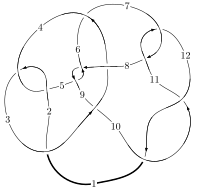
\includegraphics[width=112pt]{../../../GIT/diagram.site/Diagrams/png/2364_12n_0275.png}\\
\ \ \ A knot diagram\footnotemark}&
\allowdisplaybreaks
\textbf{Linearized knot diagam} \\
\cline{2-2}
 &
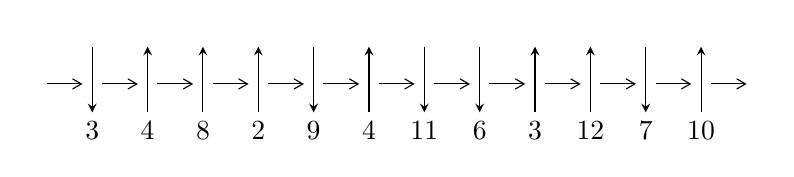
\begin{tikzpicture}[x=20pt, y=17pt]
	% nodes
	\node (C0) at (0, 0) {};
	\node (C1) at (1, 0) {};
	\node (C1U) at (1, +1) {};
	\node (C1D) at (1, -1) {3};

	\node (C2) at (2, 0) {};
	\node (C2U) at (2, +1) {};
	\node (C2D) at (2, -1) {4};

	\node (C3) at (3, 0) {};
	\node (C3U) at (3, +1) {};
	\node (C3D) at (3, -1) {8};

	\node (C4) at (4, 0) {};
	\node (C4U) at (4, +1) {};
	\node (C4D) at (4, -1) {2};

	\node (C5) at (5, 0) {};
	\node (C5U) at (5, +1) {};
	\node (C5D) at (5, -1) {9};

	\node (C6) at (6, 0) {};
	\node (C6U) at (6, +1) {};
	\node (C6D) at (6, -1) {4};

	\node (C7) at (7, 0) {};
	\node (C7U) at (7, +1) {};
	\node (C7D) at (7, -1) {11};

	\node (C8) at (8, 0) {};
	\node (C8U) at (8, +1) {};
	\node (C8D) at (8, -1) {6};

	\node (C9) at (9, 0) {};
	\node (C9U) at (9, +1) {};
	\node (C9D) at (9, -1) {3};

	\node (C10) at (10, 0) {};
	\node (C10U) at (10, +1) {};
	\node (C10D) at (10, -1) {12};

	\node (C11) at (11, 0) {};
	\node (C11U) at (11, +1) {};
	\node (C11D) at (11, -1) {7};

	\node (C12) at (12, 0) {};
	\node (C12U) at (12, +1) {};
	\node (C12D) at (12, -1) {10};
	\node (C13) at (13, 0) {};

	% arrows
	\draw[->,>={angle 60}]
	(C0) edge (C1) (C1) edge (C2) (C2) edge (C3) (C3) edge (C4) (C4) edge (C5) (C5) edge (C6) (C6) edge (C7) (C7) edge (C8) (C8) edge (C9) (C9) edge (C10) (C10) edge (C11) (C11) edge (C12) (C12) edge (C13) ;	\draw[->,>=stealth]
	(C1U) edge (C1D) (C2D) edge (C2U) (C3D) edge (C3U) (C4D) edge (C4U) (C5U) edge (C5D) (C6D) edge (C6U) (C7U) edge (C7D) (C8U) edge (C8D) (C9D) edge (C9U) (C10D) edge (C10U) (C11U) edge (C11D) (C12D) edge (C12U) ;
	\end{tikzpicture} \\
\hhline{~~} \\& 
\textbf{Solving Sequence} \\ \cline{2-2} 
 &
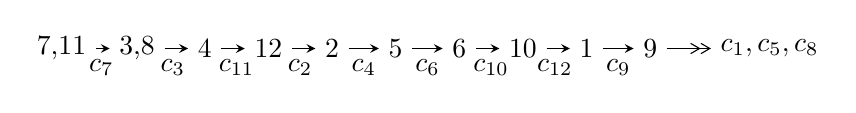
\begin{tikzpicture}[x=23pt, y=7pt]
	% node
	\node (A0) at (-1/8, 0) {7,11};
	\node (A1) at (17/16, 0) {3,8};
	\node (A2) at (17/8, 0) {4};
	\node (A3) at (25/8, 0) {12};
	\node (A4) at (33/8, 0) {2};
	\node (A5) at (41/8, 0) {5};
	\node (A6) at (49/8, 0) {6};
	\node (A7) at (57/8, 0) {10};
	\node (A8) at (65/8, 0) {1};
	\node (A9) at (73/8, 0) {9};
	\node (C1) at (1/2, -1) {$c_{7}$};
	\node (C2) at (13/8, -1) {$c_{3}$};
	\node (C3) at (21/8, -1) {$c_{11}$};
	\node (C4) at (29/8, -1) {$c_{2}$};
	\node (C5) at (37/8, -1) {$c_{4}$};
	\node (C6) at (45/8, -1) {$c_{6}$};
	\node (C7) at (53/8, -1) {$c_{10}$};
	\node (C8) at (61/8, -1) {$c_{12}$};
	\node (C9) at (69/8, -1) {$c_{9}$};
	\node (A10) at (11, 0) {$c_{1},c_{5},c_{8}$};

	% edge
	\draw[->,>=stealth]	
	(A0) edge (A1) (A1) edge (A2) (A2) edge (A3) (A3) edge (A4) (A4) edge (A5) (A5) edge (A6) (A6) edge (A7) (A7) edge (A8) (A8) edge (A9) ;
	\draw[->>,>={angle 60}]	
	(A9) edge (A10);
\end{tikzpicture} \\ 

\end{tabular} \\

\footnotetext{
The image of knot diagram is generated by the software ``\textbf{Draw programme}" developed by Andrew Bartholomew(\url{http://www.layer8.co.uk/maths/draw/index.htm\#Running-draw}), where we modified some parts for our purpose(\url{https://github.com/CATsTAILs/LinksPainter}).
}\phantom \\ \newline 
\centering \textbf{Ideals for irreducible components\footnotemark of $X_{\text{par}}$} 
 
\begin{align*}
I^u_{1}&=\langle 
-28980693473 u^{29}-23872677880 u^{28}+\cdots+214600733306 b-182162526839,\\
\phantom{I^u_{1}}&\phantom{= \langle  }-563591323347 u^{29}+759883303462 u^{28}+\cdots+214600733306 a-449269653153,\\
\phantom{I^u_{1}}&\phantom{= \langle  }u^{30}- u^{29}+\cdots+3 u+1\rangle \\
I^u_{2}&=\langle 
- u^5 a-2 u^5- u^3 a- u^2 a- u^3- a u- u^2+2 b-2 u-1,\\
\phantom{I^u_{2}}&\phantom{= \langle  }u^5 a+u^4 a+3 u^5+u^4+u^2 a+u^3+a^2+u^2+2 a+6 u+1,\;u^6+u^4+2 u^2+1\rangle \\
\\
\end{align*}
\raggedright * 2 irreducible components of $\dim_{\mathbb{C}}=0$, with total 42 representations.\\
\footnotetext{All coefficients of polynomials are rational numbers. But the coefficients are sometimes approximated in decimal forms when there is not enough margin.}
\newpage
\renewcommand{\arraystretch}{1}
\centering \section*{I. $I^u_{1}= \langle -2.90\times10^{10} u^{29}-2.39\times10^{10} u^{28}+\cdots+2.15\times10^{11} b-1.82\times10^{11},\;-5.64\times10^{11} u^{29}+7.60\times10^{11} u^{28}+\cdots+2.15\times10^{11} a-4.49\times10^{11},\;u^{30}- u^{29}+\cdots+3 u+1 \rangle$}
\flushleft \textbf{(i) Arc colorings}\\
\begin{tabular}{m{7pt} m{180pt} m{7pt} m{180pt} }
\flushright $a_{7}=$&$\begin{pmatrix}1\\0\end{pmatrix}$ \\
\flushright $a_{11}=$&$\begin{pmatrix}0\\u\end{pmatrix}$ \\
\flushright $a_{3}=$&$\begin{pmatrix}2.62623 u^{29}-3.54092 u^{28}+\cdots+12.0914 u+2.09351\\0.135045 u^{29}+0.111242 u^{28}+\cdots+0.745217 u+0.848844\end{pmatrix}$ \\
\flushright $a_{8}=$&$\begin{pmatrix}1\\u^2\end{pmatrix}$ \\
\flushright $a_{4}=$&$\begin{pmatrix}2.84774 u^{29}-3.81213 u^{28}+\cdots+12.7188 u+2.02767\\-0.0194466 u^{29}+0.399642 u^{28}+\cdots+0.672837 u+0.898553\end{pmatrix}$ \\
\flushright $a_{12}=$&$\begin{pmatrix}- u\\u\end{pmatrix}$ \\
\flushright $a_{2}=$&$\begin{pmatrix}1.18157 u^{29}-2.05139 u^{28}+\cdots+1.94907 u+0.834389\\-0.135455 u^{29}-0.0144421 u^{28}+\cdots-1.18940 u-1.25661\end{pmatrix}$ \\
\flushright $a_{5}=$&$\begin{pmatrix}1.09680 u^{29}-0.576198 u^{28}+\cdots+6.48933 u+4.12117\\-0.313730 u^{29}+0.598271 u^{28}+\cdots-1.65860 u-0.520599\end{pmatrix}$ \\
\flushright $a_{6}=$&$\begin{pmatrix}-0.947509 u^{29}+0.761849 u^{28}+\cdots-8.67784 u-0.427524\\-0.0270939 u^{29}-0.328296 u^{28}+\cdots+0.399856 u-1.39992\end{pmatrix}$ \\
\flushright $a_{10}=$&$\begin{pmatrix}- u^3\\u^3+u\end{pmatrix}$ \\
\flushright $a_{1}=$&$\begin{pmatrix}- u^5- u\\u^5+u^3+u\end{pmatrix}$ \\
\flushright $a_{9}=$&$\begin{pmatrix}1.54614 u^{29}-2.33858 u^{28}+\cdots+6.58387 u+1.61709\\-0.255461 u^{29}+0.288919 u^{28}+\cdots-1.75987 u-0.674753\end{pmatrix}$\\&\end{tabular}
\flushleft \textbf{(ii) Obstruction class $= -1$}\\~\\
\flushleft \textbf{(iii) Cusp Shapes $= -\frac{116649735226}{107300366653} u^{29}+\frac{148588842691}{107300366653} u^{28}+\cdots-\frac{788548417729}{107300366653} u+\frac{226312667156}{107300366653}$}\\~\\
\newpage\renewcommand{\arraystretch}{1}
\flushleft \textbf{(iv) u-Polynomials at the component}\newline \\
\begin{tabular}{m{50pt}|m{274pt}}
Crossings & \hspace{64pt}u-Polynomials at each crossing \\
\hline $$\begin{aligned}c_{1}\end{aligned}$$&$\begin{aligned}
&u^{30}+47 u^{29}+\cdots+191 u+1
\end{aligned}$\\
\hline $$\begin{aligned}c_{2},c_{4}\end{aligned}$$&$\begin{aligned}
&u^{30}-5 u^{29}+\cdots+11 u+1
\end{aligned}$\\
\hline $$\begin{aligned}c_{3}\end{aligned}$$&$\begin{aligned}
&u^{30}- u^{29}+\cdots+3 u+1
\end{aligned}$\\
\hline $$\begin{aligned}c_{5},c_{8}\end{aligned}$$&$\begin{aligned}
&u^{30}- u^{29}+\cdots-95 u+25
\end{aligned}$\\
\hline $$\begin{aligned}c_{6}\end{aligned}$$&$\begin{aligned}
&u^{30}+3 u^{29}+\cdots+861 u+649
\end{aligned}$\\
\hline $$\begin{aligned}c_{7},c_{11}\end{aligned}$$&$\begin{aligned}
&u^{30}+u^{29}+\cdots-3 u+1
\end{aligned}$\\
\hline $$\begin{aligned}c_{9}\end{aligned}$$&$\begin{aligned}
&u^{30}+3 u^{29}+\cdots-401099 u+75377
\end{aligned}$\\
\hline $$\begin{aligned}c_{10},c_{12}\end{aligned}$$&$\begin{aligned}
&u^{30}-5 u^{29}+\cdots-9 u+1
\end{aligned}$\\
\hline
\end{tabular}\\~\\
\newpage\renewcommand{\arraystretch}{1}
\flushleft \textbf{(v) Riley Polynomials at the component}\newline \\
\begin{tabular}{m{50pt}|m{274pt}}
Crossings & \hspace{64pt}Riley Polynomials at each crossing \\
\hline $$\begin{aligned}c_{1}\end{aligned}$$&$\begin{aligned}
&y^{30}-121 y^{29}+\cdots+51727 y+1
\end{aligned}$\\
\hline $$\begin{aligned}c_{2},c_{4}\end{aligned}$$&$\begin{aligned}
&y^{30}+47 y^{29}+\cdots+191 y+1
\end{aligned}$\\
\hline $$\begin{aligned}c_{3}\end{aligned}$$&$\begin{aligned}
&y^{30}-5 y^{29}+\cdots+11 y+1
\end{aligned}$\\
\hline $$\begin{aligned}c_{5},c_{8}\end{aligned}$$&$\begin{aligned}
&y^{30}+y^{29}+\cdots-3175 y+625
\end{aligned}$\\
\hline $$\begin{aligned}c_{6}\end{aligned}$$&$\begin{aligned}
&y^{30}+33 y^{29}+\cdots+2246675 y+421201
\end{aligned}$\\
\hline $$\begin{aligned}c_{7},c_{11}\end{aligned}$$&$\begin{aligned}
&y^{30}+5 y^{29}+\cdots+9 y+1
\end{aligned}$\\
\hline $$\begin{aligned}c_{9}\end{aligned}$$&$\begin{aligned}
&y^{30}+89 y^{29}+\cdots+64272198739 y+5681692129
\end{aligned}$\\
\hline $$\begin{aligned}c_{10},c_{12}\end{aligned}$$&$\begin{aligned}
&y^{30}+45 y^{29}+\cdots+81 y+1
\end{aligned}$\\
\hline
\end{tabular}\\~\\
\newpage\flushleft \textbf{(vi) Complex Volumes and Cusp Shapes}
$$\begin{array}{c|c|c}  
\text{Solutions to }I^u_{1}& \I (\text{vol} + \sqrt{-1}CS) & \text{Cusp shape}\\
 \hline 
\begin{aligned}
u &= \phantom{-}0.194178 + 0.861301 I \\
a &= -1.021630 - 0.362095 I \\
b &= \phantom{-}0.263501 + 0.422304 I\end{aligned}
 & \phantom{-}0.69640 - 1.72034 I & \phantom{-}1.49037 + 4.91074 I \\ \hline\begin{aligned}
u &= \phantom{-}0.194178 - 0.861301 I \\
a &= -1.021630 + 0.362095 I \\
b &= \phantom{-}0.263501 - 0.422304 I\end{aligned}
 & \phantom{-}0.69640 + 1.72034 I & \phantom{-}1.49037 - 4.91074 I \\ \hline\begin{aligned}
u &= -0.938260 + 0.627104 I \\
a &= -0.499497 + 0.926953 I \\
b &= \phantom{-}1.52482 + 0.04891 I\end{aligned}
 & -6.16879 - 1.21008 I & -2.96584 + 0.88236 I \\ \hline\begin{aligned}
u &= -0.938260 - 0.627104 I \\
a &= -0.499497 - 0.926953 I \\
b &= \phantom{-}1.52482 - 0.04891 I\end{aligned}
 & -6.16879 + 1.21008 I & -2.96584 - 0.88236 I \\ \hline\begin{aligned}
u &= -0.423018 + 0.756823 I \\
a &= \phantom{-}1.89502 - 0.68357 I \\
b &= -0.189341 - 0.657186 I\end{aligned}
 & \phantom{-}2.22190 + 4.31885 I & \phantom{-}5.85919 - 8.87008 I \\ \hline\begin{aligned}
u &= -0.423018 - 0.756823 I \\
a &= \phantom{-}1.89502 + 0.68357 I \\
b &= -0.189341 + 0.657186 I\end{aligned}
 & \phantom{-}2.22190 - 4.31885 I & \phantom{-}5.85919 + 8.87008 I \\ \hline\begin{aligned}
u &= -0.149957 + 0.853854 I \\
a &= \phantom{-}0.90254 - 1.96897 I \\
b &= -0.496999 + 0.995959 I\end{aligned}
 & \phantom{-}3.54151 - 0.51606 I & \phantom{-}10.41425 - 1.32912 I \\ \hline\begin{aligned}
u &= -0.149957 - 0.853854 I \\
a &= \phantom{-}0.90254 + 1.96897 I \\
b &= -0.496999 - 0.995959 I\end{aligned}
 & \phantom{-}3.54151 + 0.51606 I & \phantom{-}10.41425 + 1.32912 I \\ \hline\begin{aligned}
u &= \phantom{-}0.765379 + 0.893759 I \\
a &= \phantom{-}0.159784 + 1.137040 I \\
b &= -1.46119 - 0.25226 I\end{aligned}
 & -1.42212 - 2.89990 I & \phantom{-}2.16966 + 2.50499 I \\ \hline\begin{aligned}
u &= \phantom{-}0.765379 - 0.893759 I \\
a &= \phantom{-}0.159784 - 1.137040 I \\
b &= -1.46119 + 0.25226 I\end{aligned}
 & -1.42212 + 2.89990 I & \phantom{-}2.16966 - 2.50499 I\\
 \hline 
 \end{array}$$\newpage$$\begin{array}{c|c|c}  
\text{Solutions to }I^u_{1}& \I (\text{vol} + \sqrt{-1}CS) & \text{Cusp shape}\\
 \hline 
\begin{aligned}
u &= \phantom{-}0.882441 + 0.785868 I \\
a &= \phantom{-}0.28444 + 1.44916 I \\
b &= -0.835514 + 0.010950 I\end{aligned}
 & -4.43991 - 4.87528 I & -1.40537 + 4.69553 I \\ \hline\begin{aligned}
u &= \phantom{-}0.882441 - 0.785868 I \\
a &= \phantom{-}0.28444 - 1.44916 I \\
b &= -0.835514 - 0.010950 I\end{aligned}
 & -4.43991 + 4.87528 I & -1.40537 - 4.69553 I \\ \hline\begin{aligned}
u &= \phantom{-}0.633178 + 0.448369 I \\
a &= -0.204887 - 0.469950 I \\
b &= \phantom{-}0.234278 + 0.488949 I\end{aligned}
 & -0.96186 - 1.37588 I & -2.99068 + 3.21474 I \\ \hline\begin{aligned}
u &= \phantom{-}0.633178 - 0.448369 I \\
a &= -0.204887 + 0.469950 I \\
b &= \phantom{-}0.234278 - 0.488949 I\end{aligned}
 & -0.96186 + 1.37588 I & -2.99068 - 3.21474 I \\ \hline\begin{aligned}
u &= \phantom{-}0.736913 + 0.984710 I \\
a &= \phantom{-}0.273772 + 0.001505 I \\
b &= -1.135180 - 0.258754 I\end{aligned}
 & -3.71029 - 1.15996 I & -1.23536 + 0.81989 I \\ \hline\begin{aligned}
u &= \phantom{-}0.736913 - 0.984710 I \\
a &= \phantom{-}0.273772 - 0.001505 I \\
b &= -1.135180 + 0.258754 I\end{aligned}
 & -3.71029 + 1.15996 I & -1.23536 - 0.81989 I \\ \hline\begin{aligned}
u &= -0.647311 + 1.068760 I \\
a &= -0.99194 + 1.30440 I \\
b &= \phantom{-}1.71967 - 0.46050 I\end{aligned}
 & -4.58052 + 7.07309 I & -0.56937 - 6.52418 I \\ \hline\begin{aligned}
u &= -0.647311 - 1.068760 I \\
a &= -0.99194 - 1.30440 I \\
b &= \phantom{-}1.71967 + 0.46050 I\end{aligned}
 & -4.58052 - 7.07309 I & -0.56937 + 6.52418 I \\ \hline\begin{aligned}
u &= \phantom{-}1.022110 + 0.895164 I \\
a &= -0.555012 - 0.809078 I \\
b &= \phantom{-}2.44769 - 0.22730 I\end{aligned}
 & -16.7193 + 4.9302 I & -0.87414 - 1.79412 I \\ \hline\begin{aligned}
u &= \phantom{-}1.022110 - 0.895164 I \\
a &= -0.555012 + 0.809078 I \\
b &= \phantom{-}2.44769 + 0.22730 I\end{aligned}
 & -16.7193 - 4.9302 I & -0.87414 + 1.79412 I\\
 \hline 
 \end{array}$$\newpage$$\begin{array}{c|c|c}  
\text{Solutions to }I^u_{1}& \I (\text{vol} + \sqrt{-1}CS) & \text{Cusp shape}\\
 \hline 
\begin{aligned}
u &= \phantom{-}0.919420 + 1.045210 I \\
a &= -0.57144 - 1.81078 I \\
b &= \phantom{-}2.49834 + 0.28520 I\end{aligned}
 & -16.2013 - 12.0291 I & -0.14700 + 6.09920 I \\ \hline\begin{aligned}
u &= \phantom{-}0.919420 - 1.045210 I \\
a &= -0.57144 + 1.81078 I \\
b &= \phantom{-}2.49834 - 0.28520 I\end{aligned}
 & -16.2013 + 12.0291 I & -0.14700 - 6.09920 I \\ \hline\begin{aligned}
u &= -1.011130 + 0.959398 I \\
a &= \phantom{-}0.19777 - 1.52281 I \\
b &= -1.98241 + 0.56395 I\end{aligned}
 & -17.2554 + 2.6942 I & -1.35658 - 2.19435 I \\ \hline\begin{aligned}
u &= -1.011130 - 0.959398 I \\
a &= \phantom{-}0.19777 + 1.52281 I \\
b &= -1.98241 - 0.56395 I\end{aligned}
 & -17.2554 - 2.6942 I & -1.35658 + 2.19435 I \\ \hline\begin{aligned}
u &= -0.968194 + 1.019150 I \\
a &= \phantom{-}0.859717 - 0.564264 I \\
b &= -2.08559 - 0.52091 I\end{aligned}
 & -17.0465 + 4.5510 I & -1.15103 - 1.97489 I \\ \hline\begin{aligned}
u &= -0.968194 - 1.019150 I \\
a &= \phantom{-}0.859717 + 0.564264 I \\
b &= -2.08559 + 0.52091 I\end{aligned}
 & -17.0465 - 4.5510 I & -1.15103 + 1.97489 I \\ \hline\begin{aligned}
u &= -0.213905 + 0.490541 I \\
a &= -1.65502 + 0.37124 I \\
b &= -0.548040 + 0.708878 I\end{aligned}
 & \phantom{-}1.59074 - 1.61799 I & \phantom{-}1.307109 - 0.397413 I \\ \hline\begin{aligned}
u &= -0.213905 - 0.490541 I \\
a &= -1.65502 - 0.37124 I \\
b &= -0.548040 - 0.708878 I\end{aligned}
 & \phantom{-}1.59074 + 1.61799 I & \phantom{-}1.307109 + 0.397413 I \\ \hline\begin{aligned}
u &= -0.301843 + 0.271696 I \\
a &= \phantom{-}2.42638 + 1.75700 I \\
b &= -0.454022 - 0.958650 I\end{aligned}
 & \phantom{-}1.49855 + 2.22404 I & -0.54522 - 4.55103 I \\ \hline\begin{aligned}
u &= -0.301843 - 0.271696 I \\
a &= \phantom{-}2.42638 - 1.75700 I \\
b &= -0.454022 + 0.958650 I\end{aligned}
 & \phantom{-}1.49855 - 2.22404 I & -0.54522 + 4.55103 I\\
 \hline 
 \end{array}$$\newpage\newpage\renewcommand{\arraystretch}{1}
\centering \section*{II. $I^u_{2}= \langle - u^5 a-2 u^5+\cdots+2 b-1,\;u^5 a+3 u^5+\cdots+2 a+1,\;u^6+u^4+2 u^2+1 \rangle$}
\flushleft \textbf{(i) Arc colorings}\\
\begin{tabular}{m{7pt} m{180pt} m{7pt} m{180pt} }
\flushright $a_{7}=$&$\begin{pmatrix}1\\0\end{pmatrix}$ \\
\flushright $a_{11}=$&$\begin{pmatrix}0\\u\end{pmatrix}$ \\
\flushright $a_{3}=$&$\begin{pmatrix}a\\\frac{1}{2} u^5 a+u^5+\cdots+u+\frac{1}{2}\end{pmatrix}$ \\
\flushright $a_{8}=$&$\begin{pmatrix}1\\u^2\end{pmatrix}$ \\
\flushright $a_{4}=$&$\begin{pmatrix}\frac{1}{2} u^5 a+u^5+\cdots+a+\frac{1}{2}\\\frac{1}{2} u^5 a+\frac{1}{2} u^5+\cdots+u^2+\frac{1}{2}\end{pmatrix}$ \\
\flushright $a_{12}=$&$\begin{pmatrix}- u\\u\end{pmatrix}$ \\
\flushright $a_{2}=$&$\begin{pmatrix}-2 u^5-\frac{1}{2} u^4+\cdots+\frac{1}{2} a-2\\\frac{1}{2} u^4 a+\frac{3}{2} u^5+\cdots+2 u+1\end{pmatrix}$ \\
\flushright $a_{5}=$&$\begin{pmatrix}u^5+u\\- u^5- u^3- u\end{pmatrix}$ \\
\flushright $a_{6}=$&$\begin{pmatrix}\frac{1}{2} u^5 a+\frac{7}{2} u^5+\cdots+\frac{1}{2} a+\frac{5}{2}\\u^5 a-\frac{3}{2} u^5+\cdots+\frac{1}{2} a-\frac{5}{2} u\end{pmatrix}$ \\
\flushright $a_{10}=$&$\begin{pmatrix}- u^3\\u^3+u\end{pmatrix}$ \\
\flushright $a_{1}=$&$\begin{pmatrix}- u^5- u\\u^5+u^3+u\end{pmatrix}$ \\
\flushright $a_{9}=$&$\begin{pmatrix}\frac{3}{2} u^5 a+\frac{1}{2} u^5+\cdots+\frac{1}{2} a-\frac{3}{2}\\- u^5 a-\frac{5}{2} u^5+\cdots+\frac{1}{2} a-1\end{pmatrix}$\\&\end{tabular}
\flushleft \textbf{(ii) Obstruction class $= 1$}\\~\\
\flushleft \textbf{(iii) Cusp Shapes $= -2 u^5 a-2 u^3 a+4 u^4-2 u^2 a+2 u^3-2 a u+2 u^2+10$}\\~\\
\newpage\renewcommand{\arraystretch}{1}
\flushleft \textbf{(iv) u-Polynomials at the component}\newline \\
\begin{tabular}{m{50pt}|m{274pt}}
Crossings & \hspace{64pt}u-Polynomials at each crossing \\
\hline $$\begin{aligned}c_{1},c_{4}\end{aligned}$$&$\begin{aligned}
&(u^2- u+1)^6
\end{aligned}$\\
\hline $$\begin{aligned}c_{2}\end{aligned}$$&$\begin{aligned}
&(u^2+u+1)^6
\end{aligned}$\\
\hline $$\begin{aligned}c_{3}\end{aligned}$$&$\begin{aligned}
&(u^4- u^2+1)^3
\end{aligned}$\\
\hline $$\begin{aligned}c_{5},c_{8}\end{aligned}$$&$\begin{aligned}
&(u^2+1)^6
\end{aligned}$\\
\hline $$\begin{aligned}c_{6}\end{aligned}$$&$\begin{aligned}
&u^{12}-6 u^{11}+\cdots+2 u+1
\end{aligned}$\\
\hline $$\begin{aligned}c_{7},c_{11}\end{aligned}$$&$\begin{aligned}
&(u^6+u^4+2 u^2+1)^2
\end{aligned}$\\
\hline $$\begin{aligned}c_{9}\end{aligned}$$&$\begin{aligned}
&u^{12}+2 u^{11}+\cdots+4 u+1
\end{aligned}$\\
\hline $$\begin{aligned}c_{10}\end{aligned}$$&$\begin{aligned}
&(u^3+u^2+2 u+1)^4
\end{aligned}$\\
\hline $$\begin{aligned}c_{12}\end{aligned}$$&$\begin{aligned}
&(u^3- u^2+2 u-1)^4
\end{aligned}$\\
\hline
\end{tabular}\\~\\
\newpage\renewcommand{\arraystretch}{1}
\flushleft \textbf{(v) Riley Polynomials at the component}\newline \\
\begin{tabular}{m{50pt}|m{274pt}}
Crossings & \hspace{64pt}Riley Polynomials at each crossing \\
\hline $$\begin{aligned}c_{1},c_{2},c_{4}\end{aligned}$$&$\begin{aligned}
&(y^2+y+1)^6
\end{aligned}$\\
\hline $$\begin{aligned}c_{3}\end{aligned}$$&$\begin{aligned}
&(y^2- y+1)^6
\end{aligned}$\\
\hline $$\begin{aligned}c_{5},c_{8}\end{aligned}$$&$\begin{aligned}
&(y+1)^{12}
\end{aligned}$\\
\hline $$\begin{aligned}c_{6}\end{aligned}$$&$\begin{aligned}
&y^{12}+12 y^{11}+\cdots+6 y+1
\end{aligned}$\\
\hline $$\begin{aligned}c_{7},c_{11}\end{aligned}$$&$\begin{aligned}
&(y^3+y^2+2 y+1)^4
\end{aligned}$\\
\hline $$\begin{aligned}c_{9}\end{aligned}$$&$\begin{aligned}
&y^{12}-12 y^{11}+\cdots-6 y+1
\end{aligned}$\\
\hline $$\begin{aligned}c_{10},c_{12}\end{aligned}$$&$\begin{aligned}
&(y^3+3 y^2+2 y-1)^4
\end{aligned}$\\
\hline
\end{tabular}\\~\\
\newpage\flushleft \textbf{(vi) Complex Volumes and Cusp Shapes}
$$\begin{array}{c|c|c}  
\text{Solutions to }I^u_{2}& \I (\text{vol} + \sqrt{-1}CS) & \text{Cusp shape}\\
 \hline 
\begin{aligned}
u &= \phantom{-}0.744862 + 0.877439 I \\
a &= \phantom{-}0.850078 - 0.184922 I \\
b &= -0.807141 + 0.650946 I\end{aligned}
 & -1.37919 - 0.79824 I & \phantom{-}2.49024 - 0.48465 I \\ \hline\begin{aligned}
u &= \phantom{-}0.744862 + 0.877439 I \\
a &= -0.227778 + 1.317500 I \\
b &= -0.807141 - 1.081110 I\end{aligned}
 & -1.37919 - 4.85801 I & \phantom{-}2.49024 + 6.44355 I \\ \hline\begin{aligned}
u &= \phantom{-}0.744862 - 0.877439 I \\
a &= \phantom{-}0.850078 + 0.184922 I \\
b &= -0.807141 - 0.650946 I\end{aligned}
 & -1.37919 + 0.79824 I & \phantom{-}2.49024 + 0.48465 I \\ \hline\begin{aligned}
u &= \phantom{-}0.744862 - 0.877439 I \\
a &= -0.227778 - 1.317500 I \\
b &= -0.807141 + 1.081110 I\end{aligned}
 & -1.37919 + 4.85801 I & \phantom{-}2.49024 - 6.44355 I \\ \hline\begin{aligned}
u &= -0.744862 + 0.877439 I \\
a &= \phantom{-}0.317499 + 0.772222 I \\
b &= \phantom{-}1.80714 - 1.08111 I\end{aligned}
 & -1.37919 + 0.79824 I & \phantom{-}2.49024 + 0.48465 I \\ \hline\begin{aligned}
u &= -0.744862 + 0.877439 I \\
a &= -1.18492 + 1.85008 I \\
b &= \phantom{-}1.80714 + 0.65095 I\end{aligned}
 & -1.37919 + 4.85801 I & \phantom{-}2.49024 - 6.44355 I \\ \hline\begin{aligned}
u &= -0.744862 - 0.877439 I \\
a &= \phantom{-}0.317499 - 0.772222 I \\
b &= \phantom{-}1.80714 + 1.08111 I\end{aligned}
 & -1.37919 - 0.79824 I & \phantom{-}2.49024 - 0.48465 I \\ \hline\begin{aligned}
u &= -0.744862 - 0.877439 I \\
a &= -1.18492 - 1.85008 I \\
b &= \phantom{-}1.80714 - 0.65095 I\end{aligned}
 & -1.37919 - 4.85801 I & \phantom{-}2.49024 + 6.44355 I \\ \hline\begin{aligned}
u &= \phantom{-0.000000 -}0.754878 I \\
a &= \phantom{-}0.64233 - 1.64233 I \\
b &= \phantom{-}0.50000 + 1.43587 I\end{aligned}
 & \phantom{-}2.75839 + 2.02988 I & \phantom{-}9.01951 - 3.46410 I \\ \hline\begin{aligned}
u &= \phantom{-0.000000 -}0.754878 I \\
a &= -2.39721 + 1.39721 I \\
b &= \phantom{-}0.500000 - 0.296185 I\end{aligned}
 & \phantom{-}2.75839 - 2.02988 I & \phantom{-}9.01951 + 3.46410 I\\
 \hline 
 \end{array}$$\newpage$$\begin{array}{c|c|c}  
\text{Solutions to }I^u_{2}& \I (\text{vol} + \sqrt{-1}CS) & \text{Cusp shape}\\
 \hline 
\begin{aligned}
u &= \phantom{-0.000000 } -0.754878 I \\
a &= \phantom{-}0.64233 + 1.64233 I \\
b &= \phantom{-}0.50000 - 1.43587 I\end{aligned}
 & \phantom{-}2.75839 - 2.02988 I & \phantom{-}9.01951 + 3.46410 I \\ \hline\begin{aligned}
u &= \phantom{-0.000000 } -0.754878 I \\
a &= -2.39721 - 1.39721 I \\
b &= \phantom{-}0.500000 + 0.296185 I\end{aligned}
 & \phantom{-}2.75839 + 2.02988 I & \phantom{-}9.01951 - 3.46410 I\\
 \hline 
 \end{array}$$\newpage
\newpage\renewcommand{\arraystretch}{1}
\centering \section*{ III. u-Polynomials}
\begin{tabular}{m{50pt}|m{274pt}}
Crossings & \hspace{64pt}u-Polynomials at each crossing \\
\hline $$\begin{aligned}c_{1}\end{aligned}$$&$\begin{aligned}
&((u^2- u+1)^6)(u^{30}+47 u^{29}+\cdots+191 u+1)
\end{aligned}$\\
\hline $$\begin{aligned}c_{2}\end{aligned}$$&$\begin{aligned}
&((u^2+u+1)^6)(u^{30}-5 u^{29}+\cdots+11 u+1)
\end{aligned}$\\
\hline $$\begin{aligned}c_{3}\end{aligned}$$&$\begin{aligned}
&((u^4- u^2+1)^3)(u^{30}- u^{29}+\cdots+3 u+1)
\end{aligned}$\\
\hline $$\begin{aligned}c_{4}\end{aligned}$$&$\begin{aligned}
&((u^2- u+1)^6)(u^{30}-5 u^{29}+\cdots+11 u+1)
\end{aligned}$\\
\hline $$\begin{aligned}c_{5},c_{8}\end{aligned}$$&$\begin{aligned}
&((u^2+1)^6)(u^{30}- u^{29}+\cdots-95 u+25)
\end{aligned}$\\
\hline $$\begin{aligned}c_{6}\end{aligned}$$&$\begin{aligned}
&(u^{12}-6 u^{11}+\cdots+2 u+1)(u^{30}+3 u^{29}+\cdots+861 u+649)
\end{aligned}$\\
\hline $$\begin{aligned}c_{7},c_{11}\end{aligned}$$&$\begin{aligned}
&((u^6+u^4+2 u^2+1)^2)(u^{30}+u^{29}+\cdots-3 u+1)
\end{aligned}$\\
\hline $$\begin{aligned}c_{9}\end{aligned}$$&$\begin{aligned}
&(u^{12}+2 u^{11}+\cdots+4 u+1)(u^{30}+3 u^{29}+\cdots-401099 u+75377)
\end{aligned}$\\
\hline $$\begin{aligned}c_{10}\end{aligned}$$&$\begin{aligned}
&((u^3+u^2+2 u+1)^4)(u^{30}-5 u^{29}+\cdots-9 u+1)
\end{aligned}$\\
\hline $$\begin{aligned}c_{12}\end{aligned}$$&$\begin{aligned}
&((u^3- u^2+2 u-1)^4)(u^{30}-5 u^{29}+\cdots-9 u+1)
\end{aligned}$\\
\hline
\end{tabular}\newpage\renewcommand{\arraystretch}{1}
\centering \section*{ IV. Riley Polynomials}
\begin{tabular}{m{50pt}|m{274pt}}
Crossings & \hspace{64pt}Riley Polynomials at each crossing \\
\hline $$\begin{aligned}c_{1}\end{aligned}$$&$\begin{aligned}
&((y^2+y+1)^6)(y^{30}-121 y^{29}+\cdots+51727 y+1)
\end{aligned}$\\
\hline $$\begin{aligned}c_{2},c_{4}\end{aligned}$$&$\begin{aligned}
&((y^2+y+1)^6)(y^{30}+47 y^{29}+\cdots+191 y+1)
\end{aligned}$\\
\hline $$\begin{aligned}c_{3}\end{aligned}$$&$\begin{aligned}
&((y^2- y+1)^6)(y^{30}-5 y^{29}+\cdots+11 y+1)
\end{aligned}$\\
\hline $$\begin{aligned}c_{5},c_{8}\end{aligned}$$&$\begin{aligned}
&((y+1)^{12})(y^{30}+y^{29}+\cdots-3175 y+625)
\end{aligned}$\\
\hline $$\begin{aligned}c_{6}\end{aligned}$$&$\begin{aligned}
&(y^{12}+12 y^{11}+\cdots+6 y+1)(y^{30}+33 y^{29}+\cdots+2246675 y+421201)
\end{aligned}$\\
\hline $$\begin{aligned}c_{7},c_{11}\end{aligned}$$&$\begin{aligned}
&((y^3+y^2+2 y+1)^4)(y^{30}+5 y^{29}+\cdots+9 y+1)
\end{aligned}$\\
\hline $$\begin{aligned}c_{9}\end{aligned}$$&$\begin{aligned}
&(y^{12}-12 y^{11}+\cdots-6 y+1)\\
&\cdot(y^{30}+89 y^{29}+\cdots+64272198739 y+5681692129)
\end{aligned}$\\
\hline $$\begin{aligned}c_{10},c_{12}\end{aligned}$$&$\begin{aligned}
&((y^3+3 y^2+2 y-1)^4)(y^{30}+45 y^{29}+\cdots+81 y+1)
\end{aligned}$\\
\hline
\end{tabular}
\vskip 2pc
\end{document}